\subsection{BÀI TẬP TRẮC NGHIỆM}
\Opensolutionfile{ans}[ans/ans0D6-B2]

\begin{ex}%[0D2B3]
	Parabol $y=-x^2+2x$ có đỉnh là
	\choice 
	{\True $I(1;1)$}
	{$I(-1;1)$}
	{$I(-1;2)$}
	{$I(2;0)$}
	\loigiai{
		\begin{itemize}
			\item [$\bullet$] Hoành độ đỉnh $x=-\dfrac{b}{2a}=\dfrac{-2}{2 \cdot (-1)}=1$.
			\item [$\bullet$] Với $x=1$ thay vào phương trình, ta tính được $y=1$.
		\end{itemize}
	Vậy tọa độ đỉnh là $I(1;1)$.
	}
\end{ex}

\begin{ex}%[0D2B3]
	Tìm tọa độ đỉnh $I$ của Parabol $y=x^2-3x+4$.
	\choice{$I(3;3)$}
	{\True $\left(\dfrac{3}{2};\dfrac{7}{4}\right)$}
	{$\left(-\dfrac{3}{2};\dfrac{43}{4}\right)$}
	{$\left(\dfrac{3}{2};-\dfrac{7}{4}\right)$}
	\loigiai{
		\begin{itemize}
			\item [$\bullet$] Hoành độ đỉnh $x=-\dfrac{b}{2a}=\dfrac{3}{2 \cdot (1)}=\dfrac{3}{2}$.
			\item [$\bullet$] Với $x=\dfrac{3}{2}$ thay vào phương trình, ta tính được $y=\dfrac{7}{4}$.
		\end{itemize}
		Vậy tọa độ đỉnh là $\left(\dfrac{3}{2};\dfrac{7}{4}\right)$.
	}
\end{ex}


\begin{ex}%[0D2B3]
	Tìm phương trình trục đối xứng của đồ thị hàm số $y=-x^2+6x+7$.
	\choice
	{$y=6$}
	{\True $x=3$}
	{$y=3$}
	{$x=6$}
	\loigiai{
		Phương trình trục đối xứng là $x=-\dfrac{b}{2a}=3$.
	}
\end{ex}

\begin{ex}%[0D2Y3]
	Đồ thị hàm số $y=2x^2 - x - 3$ có trục đối xứng là 
	\choice
	{\True $x=\dfrac{1}{4}$}
	{$x= - \dfrac{1}{2}$}
	{$x= - \dfrac{1}{4}$}
	{$x=\dfrac{1}{2}$}
	\loigiai{
		Ta có $x=\dfrac{1}{4}$ là trục đối xứng của đồ thị $y=2x^2-x-3$.}
\end{ex}

\begin{ex}%[0D2B3]
	Điểm nào sau đây thuộc đồ thị hàm số $y = -x^2 + 4x + 1$?
	\choice
	{$M(-2;-12)$}
	{$N(1;3)$}
	{$P(-1;-5)$}
	{\True $Q(2;5)$}
	\loigiai
	{
		Bảng giá trị:
		\begin{center}
			\begin{tabular}{|c|c|c|c|c|}
				\hline
				$x$ & $-2$ & $-1$ & $1$ & $2$\\
				\hline
				$y$ & $-11$ & $-4$ & $4$ & $5$\\
				\hline
			\end{tabular}
		\end{center}
		Vậy điểm $Q(2;5)$ thuộc đồ thị hàm số $y = -x^2 + 4x + 1$.
	}
\end{ex}

\begin{ex}%[0D2B3]
	Tìm giá trị của $m$ để parabol $y=x^2+mx+1$ đi qua điểm $A(1;1)$.
	\choice
	{$m=1$}
	{$m=2$}
	{\True $m=-1$}
	{$m=-2$}
	\loigiai{
		Đồ thị hàm số $y=x^2+mx+1$ đi qua điểm $A(1;1)$ thì $1=1^2+m \cdot 1 + 1 \Leftrightarrow m=-1$.
	}
\end{ex}

\begin{ex}%[0D2B3]
	Cho hàm số $y =  - x^2 + 4x + 3$. Chọn khẳng định đúng.
	\choice
	{Hàm số đồng biến trên $\mathbb{R}$}
	{Hàm số đồng biến trên $(2, + \infty )$}
	{\True Hàm số nghịch biến trên $(2, + \infty )$}
	{Hàm số nghịch biến trên $\mathbb{R}$}
	\loigiai{
		Tọa độ đỉnh $(2;7)$.\\
		Bảng biến thiên
		\begin{center}
			
\begin{tikzpicture}
			\tkzTabInit[nocadre=false, lgt=1,espcl=3]  
			{$x$/0.8, $y$/2}  
			{$-\infty$, $2$, $+\infty$}  
			\tkzTabVar{-/ $-\infty$, +/ $7$ , -/ $-\infty$}  
			\end{tikzpicture}
		\end{center}
		Dựa vào bảng biến thiên, ta có hàm số đồng biến trên $(- \infty ,2)$ và hàm số nghịch biến trên $(2, + \infty )$.
	}
\end{ex}

\begin{ex}%[0D2B3]
	Hàm số $y=x^2+2x+2$ đồng biến trên khoảng nào dưới đây?
	\choice
	{$(-\infty; + \infty ) $}
	{$(-2;+\infty ) $}
	{\True $\left( -1; + \infty \right) $}
	{$(-\infty; -1 ) $}
	\loigiai{
		Tọa độ đỉnh $I(-1;1)$.\\
		Bảng biến thiên
		\begin{center}
			
\begin{tikzpicture}
				\tkzTabInit[nocadre=false, lgt=1,espcl=3]  
				{$x$/0.8, $y$/2}  
				{$-\infty$, $-1$, $+\infty$}  
				\tkzTabVar{+/ $+\infty$, -/ $1$ , +/ $+\infty$}  
			\end{tikzpicture}
		\end{center}
		Suy ra hàm số đồng biến trên khoảng $(-1;+\infty)$.
	}
\end{ex}

\begin{ex}%[0D2B3-1]
	Hàm số $y=-x^2+2x+3$ đồng biến trên
	\choice
	{$(-1;+\infty)$}
	{$(-\infty;-1)$}
	{$(1; +\infty)$}
	{\True $(-\infty; 1)$}
	\loigiai{
		Tọa độ đỉnh $I(1; 4)$.\\
		Ta có bảng biến thiên của hàm số đã cho như sau:
		\begin{center}
			
\begin{tikzpicture}[>=stealth]
			\tkzTabInit[lgt=1,espcl=2.5]
			{ $x$ /0.8, $y$ /2}
			{$-\infty$,$1$,$+\infty$}
			\tkzTabVar{-/$-\infty$, +/$4$, -/$-\infty$}
			\end{tikzpicture}
		\end{center}
		Từ bảng biến thiên ta thấy, hàm số đã cho đồng biến trên $(-\infty; 1)$.
	}
\end{ex}

\begin{ex}%[0D2B3]
	\immini{ 
		Đường cong trong hình vẽ bên là đồ thị của một trong các hàm số cho ở các phương án {\bf A, B, C, D}. Hỏi đó là hàm số nào?
		\motcot
		{$y=x^2-4x-3$}
		{$y=-x^2+4x$}
		{$y=x^2+4x-3$}
		{\True $y=-x^2+4x-3$}
	}{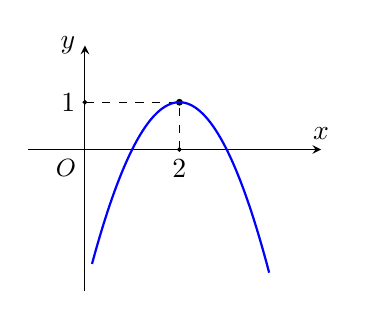
\begin{tikzpicture}[scale=0.6,>=stealth];
		\draw [black, ->] (-1.2,0)--(5,0) node [above] {$x$};
		\draw [black, ->] (0,-3)--(0,2.2) node [left] {$y$};
		\draw [dashed] (2,0)--(2,1)--(0,1);
		\draw [fill=black](2,0) node[below]{2} circle (1pt);
		\draw [fill=black](0,1) node[left]{1} circle (1pt);
		\draw [fill=black](2,1) circle (1.7pt);
		\draw[smooth,,blue,thick,samples=100,domain=0.15:3.9] plot(\x,{-(\x)^2+4*(\x)-3});
		\node at (-0.4,-0.4) {\small$O$};
		\end{tikzpicture}}
	\loigiai{Đồ thị đã cho là đồ thị của hàm số bậc hai có hệ số $a<0$, tọa độ đỉnh $I\left(2;1\right)$. Trong bốn hàm số đã cho chỉ có hàm số $y=-x^2+4x-3$ thỏa mãn tính chất về đồ thị như hình vẽ.
	}
\end{ex}

\begin{ex}%[0D2B3]
	\immini{Hình bên là đồ thị của một hàm số bậc hai. Hàm số đó là hàm số nào trong các hàm số sau?
		\choice
		{$ y =  - {x^2} + 3x - 1 $}
		{$y =  - 2{x^2} + 3x - 1$}
		{\True $y = 2{x^2} - 3x + 1$}
		{$y = {x^2} - 3x + 1$} }{
		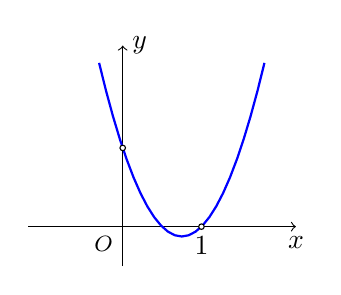
\begin{tikzpicture}
		\draw[->] (-1.2,0) -- (2.2,0) node[below] {$x$};
		\draw[->] (0,-0.5) -- (0,2.3) node[right] {$y$};
		\node at (0,0) [below left] {\footnotesize $O$};
		\draw [domain=-0.3:1.8,blue,thick] plot (\x, {2*((\x)^2)-3*(\x)+1)} );
		\node at (1,0) [below]{$1$};
		\fill[fill=white,draw=black]
		(1,0) circle (1pt) (0,1) circle (1pt);
		\end{tikzpicture}}
	\loigiai{
		\begin{itemize}
			\item [$\bullet$] Phía phải đồ thị đi lên nên $a>0$, ta loại các phương án có hệ số $a<0$.
			\item [$\bullet$] Đồ thị hàm số qua điểm $(1;0)$ nên chỉ có phương án $y = 2{x^2} - 3x + 1$ thỏa mãn.
		\end{itemize}
	}
\end{ex}

\begin{ex}%[0D2B3]
	\immini{Hàm số nào trong các hàm số sau đây có bảng biến thiên như hình vẽ
		\choice
		{\True $y = -x^2 + 2x -3$}
		{$y = x^2 +2x -1 $}
		{$y = -x^2 -x -1$}
		{$y = x^2 -x -1$}
	}{\hspace{1cm}
		
\begin{tikzpicture}
		\tkzTabInit[nocadre=false, lgt=0.8, espcl=2]{$x$ /0.7,$y$ /1.4}{$-\infty$,$1$,$+\infty$}
		\tkzTabVar{-/ $-\infty$ / ,+/$-2$, -/ $-\infty$ /}
		\end{tikzpicture}}
	\loigiai{
	\begin{itemize}
		\item [$\bullet$] Phía phải đồ thị đi xuống nên $a<0$, ta loại các phương án có hệ số $a>0$.
		\item [$\bullet$] Đồ thị hàm số qua điểm $(1;-2)$ nên chỉ có phương án $y = -x^2 + 2x -3$ thỏa mãn.
	\end{itemize}
	}
\end{ex}

\begin{ex}%[0D2B3-1]
	Bảng biến thiên của hàm số $y=-2x^2+4x+1$ là bảng nào sau đây?
	\choice
	{
\begin{tikzpicture}
		\tkzTabInit
		[lgt=0.7,espcl=1.9] % tùy chọn
		{$x$/0.7, $y$/1.2} % cột đầu tiên
		{$-\infty$, $2$, $+\infty$} % hàng 1 cột 2
		%\tkzTabLine{,-,0,+,} % hàng 2 cột 2
		\tkzTabVar{+/ $+\infty$, -/ $1$ , +/ $+\infty$} % hàng 3 cột 2
		\end{tikzpicture}}
	{\True 
\begin{tikzpicture}
		\tkzTabInit
		[lgt=0.7,espcl=1.9] % tùy chọn
		{$x$/0.7, $y$/1.2} % cột đầu tiên
		{$-\infty$, $1$, $+\infty$} % hàng 1 cột 2
		%\tkzTabLine{,-,0,+,} % hàng 2 cột 2
		\tkzTabVar{-/ $-\infty$, +/ $3$ , -/ $-\infty$} % hàng 3 cột 2
		\end{tikzpicture}}
	{
\begin{tikzpicture}
		\tkzTabInit
		[lgt=0.7,espcl=1.9] % tùy chọn
		{$x$/0.7, $y$/1.2} % cột đầu tiên
		{$-\infty$, $2$, $+\infty$} % hàng 1 cột 2
		%\tkzTabLine{,-,0,+,} % hàng 2 cột 2
		\tkzTabVar{-/ $-\infty$, +/ $1$ , -/ $-\infty$} % hàng 3 cột 2
		\end{tikzpicture}}
	{
\begin{tikzpicture}
		\tkzTabInit
		[lgt=0.7,espcl=1.9] % tùy chọn
		{$x$/0.7, $y$/1.2} % cột đầu tiên
		{$-\infty$, $1$, $+\infty$} % hàng 1 cột 2
		%\tkzTabLine{,-,0,+,} % hàng 2 cột 2
		\tkzTabVar{+/ $+\infty$, -/ $3$ , +/ $+\infty$} % hàng 3 cột 2
		\end{tikzpicture}}
	\loigiai{
		Tọa độ đỉnh $I(1;3)$ và $a = -2 < 0$ nên bảng biến thiên như sau
		\begin{center}
			
\begin{tikzpicture}
			\tkzTabInit
			[lgt=0.7,espcl=1.5] % tùy chọn
			{$x$/0.7, $y$/1.2} % cột đầu tiên
			{$-\infty$, $1$, $+\infty$} % hàng 1 cột 2
			%\tkzTabLine{,-,0,+,} % hàng 2 cột 2
			\tkzTabVar{-/ $-\infty$, +/ $3$ , -/ $-\infty$} % hàng 3 cột 2
			\end{tikzpicture}
		\end{center}
	}
	
\end{ex}


\begin{ex}%[0D2B3-3]
	Gọi $S$ là tập giá trị của hàm số $y=-x^2+4x$. Hỏi tập $S$ có bao nhiêu số nguyên dương?
	\choice
	{$5$}
	{\True $4$}
	{$3$}
	{$0$}
	\loigiai{
		Tọa độ đỉnh của parabol $(P)$ này là $\left(2; 4 \right)$. Suy ra $S=(-\infty;4]$.\\
		Tập $S$ có 4 số nguyên dương là 1, 2, 3, 4.
	}
\end{ex}

\begin{ex}%[0D2B3-1]
	Giá trị nhỏ nhất của hàm số $y=x^2-2x+3$ bằng
	\choice 
	{$0$}
	{$3$}
	{$1$}
	{\True $2$}
	\loigiai{Ta có $y=x^2-2x+3=(x-1)^2+2 \ge 2$. Đẳng thức xảy ra khi 
		$x=1$. Vậy $\min y = 2$.
	}	
\end{ex}

\begin{ex}%[0D2B3-1]
	Giá trị lớn nhất của hàm số $y=-x^2-2x+4$ là
	\choice
	{\True $5$}
	{$1$}
	{$-1$}
	{$3$}
	\loigiai{
		Ta có
		\[-x^2-2x+4=-(x+1)^2+5\le 5\ ,\forall x\in\mathbb{R}.\]
		Đẳng thức xảy ra khi $x=-1$. Vậy giá trị lớn nhất của hàm số đã cho là $5$.
	}
\end{ex}

\begin{ex}%[0D2B3-4]
	Giao điểm của parabol $(P) \colon y = x^2-3x-4$ với trục tung là
	\choice
	{$(4; 0)$}
	{\True $(0; -4)$}
	{$(0; -1)$}
	{$(-1; 0)$}
	\loigiai{
		Tọa độ giao điểm của parabol $(P)$ với trục tung là nghiệm của hệ: $\heva{&y=x^2-3x-4\\&x=0} \Leftrightarrow \heva{&x=0\\&y=-4}$.\\
		Vậy tọa độ giao điểm là $(0; -4)$.
	}
\end{ex}

\begin{ex}%[0D2B3-4]
	Giao điểm của parabol $(P) \colon y = x^2-3x-4$ với trục hoành có hoành độ lần lượt là $x_1$ và $x_2$. Tính $x_1+x_2$.
	\choice
	{$x_1+x_2=-3$.}
	{\True $x_1+x_2=3$.}
	{$x_1+x_2=4$.}
	{$x_1+x_2=-4$.}
	\loigiai{
		Xét phương trình $x^2-3x-4=0 \Leftrightarrow x_1=-1$, $x_2=4$. Suy ra $x_1+x_2=3$.
	}
\end{ex}

\begin{ex}%[0D2B3]
	Parabol $y=x^2-ax+b$ có đỉnh $I(2;-2)$. Khi đó giá trị của $a+2b$ là
	\choice
	{$a+2b=0$}
	{\True $a+2b=8$}
	{$a+2b=-2$}
	{$a+2b=4$}
	\loigiai{
		Trục đối xứng của parabol là $x=2 \Leftrightarrow \dfrac{a}{2\cdot 1}=2 \Leftrightarrow a=4$\\
		Đỉnh $I(2;-2)$ thuộc parabol nên $-2=2^2-2\cdot a +b\Leftrightarrow -2a+b=-6\Rightarrow b = 2$.\\
		Suy ra $a+2b=8$.
	}
\end{ex}

\begin{ex}%[0D2B3-2]
	\immini{
		Cho hàm số $y=ax^2+bx+c$ có đồ thị là một Parabol $(P)$ như hình vẽ bên. Trong các mệnh đề sau, mệnh đề nào là mệnh đề đúng?
		\choice
		{$a>0$, $b>0$ và $c>0$}
		{$a<0$, $b<0$ và $c>0$}
		{$a>0$, $b>0$ và $c<0$}
		{\True $a>0$, $b<0$ và $c>0$}	
	}{
		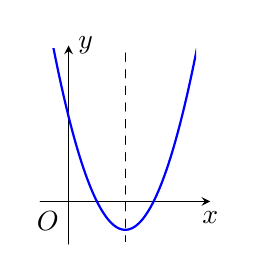
\begin{tikzpicture}[>=stealth,scale=0.6, line join=round, line cap=round,scale=0.6]
		\def\a{1} \def\b{-4} \def\c{3} % Hệ số
		\def\xmin{-1} \def\xmax{5} \def\ymin{-1.5} \def\ymax{5.5}
		\draw[->] (\xmin,0)--(\xmax,0) node [below]{$x$};
		\draw[->] (0,\ymin)--(0,\ymax) node [right]{$y$};
		\node at (0,0) [below left]{$O$};
		\clip (\xmin+0.1,\ymin+0.1) rectangle (\xmax-0.5,\ymax-0.1);
		\draw[smooth,blue,thick,samples=300] plot(\x,{\a*(\x)^2+\b*(\x)+\c});
		\draw[dashed](2,-1.5)--(2,5.5);
		\end{tikzpicture}
	}
	\loigiai{
		Chiều Parabol quay lên nên hệ số $a>0$, đồ thị hàm số cắt trục $Oy$ tại điểm ở phía trên $Ox$ nên $c>0$, trục đối xứng nằm bên phải $Oy$ nên $a, b$ trái dấu.
	}
\end{ex}

\begin{ex}%[0D2K3]
	\immini{Cho parabol $y=ax^2+bx+c$ có đồ thị như hình bên. Hãy chọn khẳng định đúng khi nói về dấu của các hệ số $a,\,b,\,c$.
	\choice 
		{$a<0,\,b>0,\,c<0$}
		{$a>0,\,b>0,\,c<0$}
		{\True $a>0,\,b<0,\,c<0$}
		{$a>0,\,b>0,\,c>0$}}
	{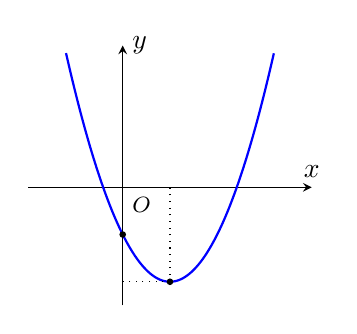
\begin{tikzpicture}[>=stealth,scale=0.6] 
		\draw[->,black] (-2,0) -- (4,0)node[above] {$x$};
		\draw[->,black] (0,-2.5) -- (0,3)node[right] {$y$}; 
		\node at (0,0) [below right] {\footnotesize $O$}; 
		\draw[smooth,blue,thick,samples=100,domain=-1.2:3.2] plot(\x,{(\x)^2-2*(\x)-1}); 
		\draw[dotted] 
		(1,-2) -- (1,0) (1,-2) -- (0,-2);
		\fill[fill=black] 
		(1,-2) circle (2pt)
		(0,-1) circle (2pt);
		\end{tikzpicture}}
	
	\loigiai
	{
		Dựa vào dạng đồ thị suy ra $ a > 0; $\\
		Giao điểm với trục $ Oy $ có tung độ âm $ \Rightarrow c < 0; $\\
		Đỉnh của $ (P) $ có hoành độ dương nên $ -\dfrac{b}{2a} > 0  $ hay $ b < 0.$\\
		Vậy $ a > 0, b < 0, c < 0. $
	}
\end{ex}


\begin{ex}%[0D2K3]
	Xác định parabol $(P):y=ax^2+bx+c$  biết $(P)$ có giá trị lớn nhất bằng $3$ tại $x=2$ và cắt trục $Ox$ tại điểm có hoành độ bằng $1$.
	\choice
	{ $y=-x^2+4x-3$}
	{ $y=x^2-4x+7$}
	{ $y=2x^2-12x+20$}
	{\True  $y=-3x^2+12x-9$}
	\loigiai
	{Theo giả thuyết suy ra đỉnh của $ (P) $ là $ I(2;3) $; $ (P) $ cắt trục hoành tại điểm có hoành độ bằng 1 nên $ (P)  $ qua $ M(1;0) $.\\
		Ta được hệ phương trình $ \heva{a+b+c=0\\-\dfrac{b}{2a} = 2\\4a + 2b + c = 3} \Leftrightarrow \heva{&a&+&b&+c &= 0\\ &4a &+&b{}&{} &= 0\\&4a &+&2b &+c &= 3} \Leftrightarrow \heva{&a = -3\\&b=12\\&c=-9.} $\\
		Vậy $ (P) $ cần tìm là: $y=-3x^2+12x-9.  $
	}
\end{ex}

\begin{ex}%[0D2K3]
	Biết parabol $(P) : y = ax^2 +bx + c$ đi qua hai điểm $A(1; 2)$ và $B(2;6)$. Tính giá trị của biểu thức $Q=3a + b$.
	\choice{\True $Q=4$}
	{$Q=-4$}
	{$Q=0$}
	{Không đủ dữ liệu để tính}
	\loigiai{
		Vì $A(1;2)$ và $B(2;6)$ nằm trên $(P)$ nên $\heva{& a+b+c=2\\ &4a+2b+c=6}\Rightarrow 3a+b=4$.
	}
\end{ex}

\begin{ex}%[0D2K3]
	Tìm $m$ để hàm số $y=x^2-2x+2m+3$ có giá trị nhỏ nhất trên đoạn $[2;5]$ bằng $-3$.
	\choice        
	{\True $m=-3$}
	{$m=-9$}
	{$m=1$}
	{$m=0$}
	\loigiai{
		\immini{Dựa vào bảng biên thiên ta có\\
			$\underset{x\in [2;5]}\min y=y(2)=2m+3$.\\
			Vậy $2m+3=-3\Rightarrow m=-3$.}{
\begin{tikzpicture}
			\tkzTabInit[nocadre=true,lgt=1,espcl=2]
			{$x$ /1,$y$ /2}{$-\infty$,$1$,$+\infty$}
			\tkzTabVar{+/ $+\infty$ ,-/$y(1)$,+/$+\infty$}
			\end{tikzpicture}}	
	}
\end{ex}

\begin{ex}%[0D2K3-5]%
	\immini{
		Một vật chuyển động trong $3$ giờ với vận tốc $v$(km/h) phụ thuộc thời gian $t$(h) có đồ thị là một phần của đường parabol có đỉnh $I(2;9)$ và trục đối xứng song song với trục tung như hình vẽ. Vận tốc tức thời của vật tại thời điểm $2$ giờ $30$ phút sau khi vật bắt đầu chuyển động gần bằng giá trị nào nhất trong các giá trị sau?
		\haicot
		{$8{,}6$(km/h)}
		{\True $8{,}8$(km/h)}
		{$8{,}5$(km/h)}
		{$8{,}7$(km/h)}
	}{
		\begin{tikzpicture}[scale=0.7, font=\footnotesize, line join=round, line cap=round, >=stealth,x=1cm,y=0.6cm]
			\def\a{-0.75} \def\b{3} \def\c{6} % Hệ số
			\def\xt{-0.6} \def\xp{4} \def\yt{10} \def\yd{-1} % x_trái, x_phải, y_trên, y_dưới (giới hạn)
			\draw[->] (\xt,0)--(\xp,0) node [below]{$t$};
			\draw[->] (0,\yd)--(0,\yt) node [right]{$v$};
			\node at (0,0) [below left]{$O$};
			\clip (\xt-0.1,\yd+0.1) rectangle (\xp-0.1,\yt-0.1);
			\draw[smooth,samples=300] plot[domain=0:3](\x,{\a*(\x)^2+\b*(\x)+\c});
			\draw[dashed] (0,9)node[left]{$9$}--(2,9)--(2,0)node[below]{$2$};
			\draw[dashed] (3,8.25)--(3,0)node[below]{$3$};
			\node at (0,6) [left]{$6$};
			\node at (2,9) [above]{$I$};
			\fill (0,0) circle (1pt) (0,6) circle (1pt) (0,9) circle (1pt) (2,0) circle (1pt) (3,0) circle (1pt);
			\fill (2,9) circle (1pt);
		\end{tikzpicture}
	}
	\loigiai{
		\immini{
			Giả sử vận tốc của vật chuyển động có phương trình là $v(t)=at^2+bt+c$.\\
			Ta có $v(2)=9\Leftrightarrow 4a+2b+c=9$; $v(0)=6\Leftrightarrow c=6$.\\
			Lại có $\heva{& \dfrac{-b}{2a}=2 \\ & 4a+2b+6=9}\Leftrightarrow
			\heva{& 4a+b=0 \\ & 4a+2b=3}\Leftrightarrow
			\heva{& a=\dfrac{-3}{4} \\ & b=3}$.\\
			Do đó $v(t)=\dfrac{-3}{4}t^2+3t+6$.\\
			Vậy $v(2{,}5)=8{,}8125$.
		}{
			\begin{tikzpicture}[scale=0.7, font=\footnotesize, line join=round, line cap=round, >=stealth,x=1cm,y=0.6cm]
				\def\a{-0.75} \def\b{3} \def\c{6} % Hệ số
				\def\xt{-0.6} \def\xp{4} \def\yt{10} \def\yd{-1} % x_trái, x_phải, y_trên, y_dưới (giới hạn)
				\draw[->] (\xt,0)--(\xp,0) node [below]{$t$};
				\draw[->] (0,\yd)--(0,\yt) node [right]{$v$};
				\node at (0,0) [below left]{$O$};
				\clip (\xt-0.1,\yd+0.1) rectangle (\xp-0.1,\yt-0.1);
				\draw[smooth,samples=300] plot[domain=0:3](\x,{\a*(\x)^2+\b*(\x)+\c});
				\draw[dashed] (0,9)node[left]{$9$}--(2,9)--(2,0)node[below]{$2$};
				\draw[dashed] (3,8.25)--(3,0)node[below]{$3$};
				\node at (0,6) [left]{$6$};
				\node at (2,9) [above]{$I$};
				\fill (0,0) circle (1pt) (0,6) circle (1pt) (0,9) circle (1pt) (2,0) circle (1pt) (3,0) circle (1pt);
				\fill (2,9) circle (1pt);
			\end{tikzpicture}
		}
	}
\end{ex}

\begin{ex}%[0D2G3-5]%
	Dây truyền đỡ trên cầu treo có dạng Parabol $ACB$ như hình vẽ.
	\begin{center}
		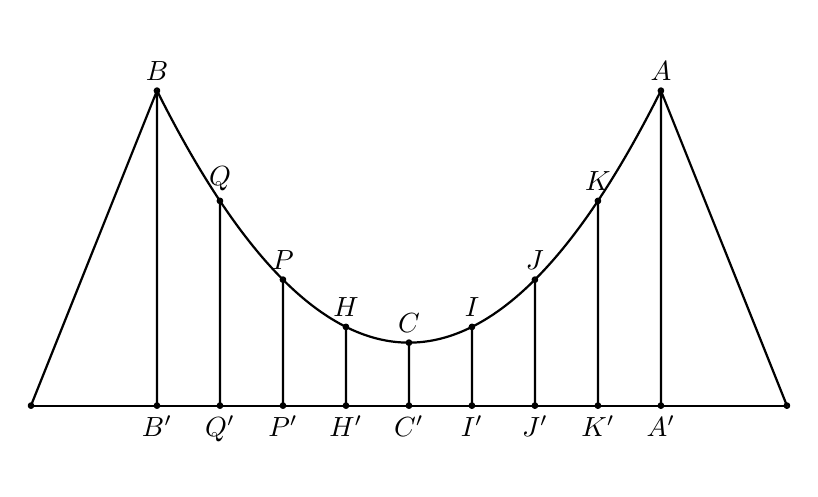
\begin{tikzpicture}[line join=round, line cap=round,>=stealth,thick,scale=.8]
			\tikzset{label style/.style={font=\footnotesize}}
			\draw[-] (-6,0)--(6,0);
			\draw (1,0)--(1,1.25) (-1,0)--(-1,1.25) (-2,0)--(-2,2) (2,0)--(2,2)
			(-3,0)--(-3,3.25) (3,0)--(3,3.25) (-4,0)--(-4,5) (4,0)--(4,5)
			(-6,0)--(-4,5) (6,0)--(4,5) (0,0)--(0,1);
			\draw (0,1) circle (1pt)node [above] {$C$} (0,0) circle (1pt) node [below] {$C'$};
			\draw (1,0) circle (1pt)node [below] {$I'$} (1,1.25) circle (1pt) node [above] {$I$};
			\draw (-1,0) circle (1pt)node [below] {$H'$} (-1,1.25) circle (1pt) node [above] {$H$};
			\draw (-2,0) circle (1pt)node [below] {$P'$} (-2,2) circle (1pt) node [above] {$P$};
			\draw (2,0) circle (1pt)node [below] {$J'$} (2,2) circle (1pt) node [above] {$J$};
			\draw (-3,0) circle (1pt)node [below] {$Q'$} (-3,3.25) circle (1pt) node [above] {$Q$};
			\draw (3,0) circle (1pt)node [below] {$K'$} (3,3.25) circle (1pt) node [above] {$K$};
			\draw (-4,0) circle (1pt)node [below] {$B'$} (-4,5) circle (1pt) node [above] {$B$};
			\draw (4,0) circle (1pt)node [below] {$A'$} (4,5) circle (1pt) node [above] {$A$};
			\draw (-6,0) circle (1pt) (6,0) circle (1pt);
			\begin{scope}
				\clip (-4,-1) rectangle (4,6);
				\draw[samples=200,domain=-4:4,smooth,variable=\x] plot (\x,{0.25*(\x)^2+1});
			\end{scope}
		\end{tikzpicture}
	\end{center}
	Đầu, cuối của dây được gắn vào các điểm $A$, $B$ trên mỗi trục $AA'$ và $BB'$ với độ cao $30$m. Chiều dài đoạn $A'B'$ trên nền cầu bằng $200$m. Độ cao ngắn nhất của dây truyền trên cầu là $OC=5$m. Gọi $Q'$, $P'$, $H'$, $O$, $I'$, $J'$, $K'$ là các điểm chia đoạn $A'B'$ thành các phần bằng nhau. Các thanh thẳng đứng nối nền cầu với đáy dây truyền: $QQ'$, $PP'$, $HH'$, $OC$, $II'$, $JJ'$, $KK'$ gọi là các dây cáp treo. Tính tổng độ dài của các dây cáp treo?
	\choice
	{\True $78,75$m}
	{$36,87$m}
	{$76,75$m}
	{$73,75$m}
	\loigiai{
		\begin{center}
			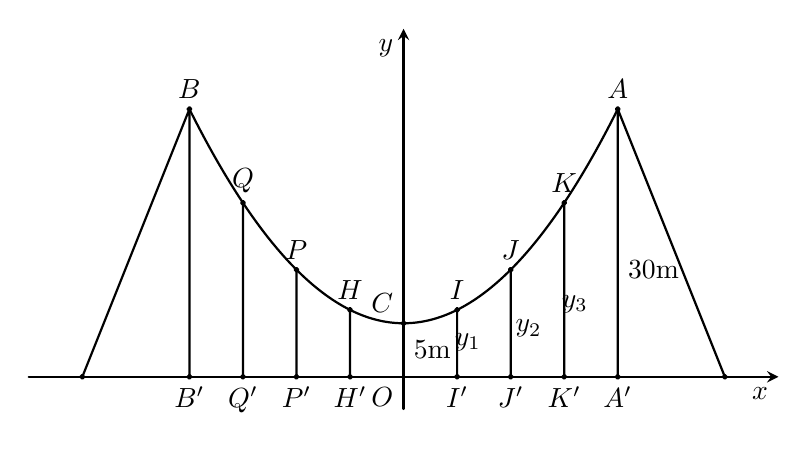
\begin{tikzpicture}[line join=round, line cap=round,>=stealth,thick,scale=.68]
				\tikzset{label style/.style={font=\footnotesize}}
				\draw[->] (-7,0)--(7,0) node[below left] {$x$};
				\draw[->] (0,-0.6)--(0,6.5) node[below left] {$y$};
				\draw (0,0) node [below left] {$O$};
				\draw (1,0)--(1,1.25) (-1,0)--(-1,1.25)
				(-2,0)--(-2,2) (2,0)--(2,2) (-3,0)--(-3,3.25) (3,0)--(3,3.25)
				(-4,0)--(-4,5) (4,0)--(4,5) (-6,0)--(-4,5) (6,0)--(4,5);
				\draw (0,1) circle (1pt)node [above left] {$C$};
				\draw (1,0) circle (1pt)node [below] {$I'$} (1,1.25) circle (1pt) node [above] {$I$};
				\draw (0,.5) node [right] {$5$m} (1.2,.3) node [above] {$y_1$};
				\draw (1.9,.9) node [right] {$y_2$} (3.2,1) node [above] {$y_3$};
				\draw (4,2) node [right] {$30$m};
				\draw (-1,0) circle (1pt)node [below] {$H'$} (-1,1.25) circle (1pt) node [above] {$H$};
				\draw (-2,0) circle (1pt)node [below] {$P'$} (-2,2) circle (1pt) node [above] {$P$};
				\draw (2,0) circle (1pt)node [below] {$J'$} (2,2) circle (1pt) node [above] {$J$};
				\draw (-3,0) circle (1pt)node [below] {$Q'$} (-3,3.25) circle (1pt) node [above] {$Q$};
				\draw (3,0) circle (1pt)node [below] {$K'$} (3,3.25) circle (1pt) node [above] {$K$};
				\draw (-4,0) circle (1pt)node [below] {$B'$} (-4,5) circle (1pt) node [above] {$B$};
				\draw (4,0) circle (1pt)node [below] {$A'$} (4,5) circle (1pt) node [above] {$A$};
				\draw (-6,0) circle (1pt) (6,0) circle (1pt);
				\begin{scope}
					\clip (-4,-1) rectangle (4,6);
					\draw[samples=200,domain=-4:4,smooth,variable=\x] plot (\x,{0.25*(\x)^2+1});
				\end{scope}
			\end{tikzpicture}
		\end{center}
		Giả sử Parabol có dạng: $y=ax^2+bx+c$, $\ a\ne 0$.\\
		Chọn hệ trục $Oxy$ như hình vẽ, khi đó parabol đi qua điểm $A\left(100;30\right)$, và có đỉnh $C(0;5)$. \\Đoạn $AB$ chia làm $8$ phần, mỗi phần $25$m.\\
		Suy ra:$\left\{\begin{aligned}
			&30=10000a+100b+c\\
			&\dfrac{-b}{2a}=0\\
			&5=c\\
		\end{aligned}\right. $ $ \Leftrightarrow \left\{\begin{aligned}
			&a=\dfrac{1}{400}\\
			&b=0\\
			&c=5\\
		\end{aligned}\right. $ $ \Rightarrow (P)\colon y=\dfrac{1}{400}x^2+5$.\\
		Gọi $T$ là tổng độ dài của các dây cáp treo. Khi đó,\\ $$\begin{aligned}
			T&=OC+2y_1+2y_2+2y_3\\
			&=5+2\left(\dfrac{1}{400}\cdot 25^2+5\right)+2\left(\dfrac{1}{400}\cdot 50^2+5\right)+2\left(\dfrac{1}{400}\cdot 75^2+5\right)\\
			&=78,75\text{m}.\end{aligned}$$}
\end{ex}

\begin{ex}
	Nhảy bungee là một trò chơi mạo hiểm. Trong trò chơi này, người chơi đứng ở vị trí trên cao, thắt dây an toàn và nhảy xuống. Sợi dây này có tính đàn hồi và được tính toán chiều dài để nó kéo người chơi lại khi gần chạm đất (hoặc mặt nước).\\
	Chiếc cầu trong hình bên dưới có bộ phận chống đỡ dạng parabol. Một người muốn thực hiện một cú nhảy bungee từ giữa cầu xuống với dây an toàn. Người này cần trang bị sợi dây an toàn dài tối đa bao nhiêu mét? Biết rằng chiều dài của sợi dây đó bằng một phần ba khoảng cách từ vị trí bắt đầu nhảy đến mặt nước.
	\begin{center}
		\begin{tikzpicture}[font=\small , line width=1pt,  >=Stealth, scale=0.8]
			\def\drong{3}
			\def\dronga{2.8}
			
			\clip ($(0,0)+(-3.6,-0.2)$) rectangle ($(0,0)+(3.6,4.7)$);
			
			\path (0,0)coordinate(O);
			
			
			
			\filldraw [orange!70!red!80!black, draw=black] ($(O)+(35:\drong)$)coordinate(A1) arc (35:145:{\drong} and {\drong})coordinate(A2) -- ($(O)+(145:\dronga)$)coordinate(A3) arc (145:35:{\dronga} and {\dronga})coordinate(A4) -- cycle;
			\foreach \a in {0,1,...,21}{
				\draw ($(O)+(35+5*\a:\drong)$)coordinate(B\a)
				($(O)+(40+5*\a:\drong)$)coordinate(D\a)
				($(O)+(37.5+5*\a:\dronga)$)coordinate(C\a) ;
				\draw (B\a)--(C\a)  (D\a)--(C\a)   ;
			}
			
			\path (A1)--++(92:1.4)coordinate(AB1)
			($(A1)+(-0.2,0)$)coordinate(AB0)--++(88:1.4)coordinate(AB2)
			;	
			\filldraw [orange!70!red!80!black, draw=black] (A1)--(AB1)--(AB2)--(AB0)--cycle; 
			\foreach \b in {0,1,...,6}{
				\draw ($(A1)!\b*0.2 cm!(AB1)$)coordinate(E\b)
				($(A1)!6+\b*0.2 cm!(AB1)$)coordinate(F\b)
				($(AB0)!2+\b*0.2 cm!(AB2)$)coordinate(G\b)
				(E\b) -- (G\b) 
				(F\b) -- (G\b) 
				;}
			%% Cột trụ 2
			\path (A2)--++(88:1.4)coordinate(AB3)
			($(A2)+(0.2,0)$)coordinate(AB4)--++(92:1.4)coordinate(AB5)
			;	
			\filldraw [orange!70!red!80!black, draw=black] (A2)--(AB3)--(AB5)--(AB4)--cycle; 
			\foreach \b in {0,1,...,6}{
				\draw ($(A2)!\b*0.2 cm!(AB3)$)coordinate(E\b)
				($(A2)!6+\b*0.2 cm!(AB3)$)coordinate(F\b)
				($(AB4)!2+\b*0.2 cm!(AB5)$)coordinate(G\b)
				(E\b) -- (G\b) 
				(F\b) -- (G\b) 
				;}
			
			
			
			%% CẦU NGANG
			\path ($(O)+(90:\drong)$)coordinate(O1)
			($(O1)+(0:4)$)coordinate(M1)
			($(O1)+(180:4)$)coordinate(M4)
			($(M1)+(90:0.2)$)coordinate(M2)
			($(M4)+(90:0.2)$)coordinate(M3)
			;
			\fill [orange!70!red!80!black, draw=black] (M1) -- (M2) -- (M3)--(M4) -- cycle;
			
			\foreach \c in {0,1,...,39}{
				\draw ($(M1)!\c*0.2 cm!(M4)$)coordinate(N\c)
				($(M2)!3+\c*0.2 cm!(M3)$)coordinate(K\c)
				($(M1)!6+\c*0.2 cm!(M4)$)coordinate(H\c)
				(N\c) -- (K\c)
				(H\c) -- (K\c) ;}
			
			%% hai bờ
			\shade [top color = green!70!blue!85!black, bottom color = brown] (M3)..controls+(30:1)and+(135:2)..($(O)+(-1.45,0.6)$) --++(240:2)--++(-1.5,0) --cycle
			;
			\shade [top color = green!70!blue!85!black , bottom color = brown]
			(M2)..controls+(150:1)and+(45:2)..($(O)+(1.45,0.6)$)--++(-60:2)--++(1.5,0)--cycle
			;
			\shade [top color = blue!40!cyan, bottom color = cyan!70!blue!30]
			($(O)+(-1.45,0.6)$) --++(240:2) -- ($(O)+(1.45,0.6)+(-60:2)$) -- ($(O)+(1.45,0.6)$) --cycle;
			\draw [<->, blue!90!black] (A2) -- ($(A2)!0.3!(A1)$)node[midway,below]{$50\,m$} ;
			\draw [<->, blue!90!black] (A1) -- ($(A2)!0.3!(A1)$)coordinate(O3)node[midway,above]{$120\,m$} ;
			\draw [<->, blue!90!black] (O3)--++(90:1.15)node[midway,right]{$45\,m$} ;	
			\draw [<->, blue!90!black] ($(A2)!0.5!(A1)$)--++(-90:1.2)node[midway,right]{$43\,m$} ;
			\draw [<->,line width=0.054pt, blue!90!black] (O1)--++(90:0.2) ;
			
			\filldraw [black] ($(O1)+(90:0.25)$) circle (0.05) ;
			\draw ($(O1)+(90:0.25)$)--++(150:1)node[left]{Vị trí nhảy} ;
			
			\draw [yellow] ($(O1)+(90:0.1)$) circle (0.1cm) ;
			\draw [yellow] ($(O1)+(30:2)$)coordinate(T1) circle (0.4cm)
			($(O1)+(90:0.2)$) -- ($(T1)+(120:0.4)$) 
			($(O1)+(90:0.0)$) -- ($(T1)+(-60:0.4)$) ;
			
			\begin{scope}
				\clip (T1) circle (0.4cm) ;
				\fill [orange!70!red!80!black] (T1) circle (0.4);
				\draw [line width=2pt] ($(T1)+(-90:0.4)$) --++(120:0.9)
				($(T1)+(-90:0.4)$) --++(60:0.9)
				;
				\draw [<->, blue] ($(T1)+(-90:0.4)$) -- ($(T1)+(90:0.4)$) ;
			\end{scope}
			\draw [blue] (T1)node[right=5pt]{$1\,m$} ;
			
			\draw [blue] (A1) arc (35:145:{\drong} and {\drong}) ;
			
		\end{tikzpicture}
	\end{center}
\choice
{\True $33$ m}
{$37$ m}
{$28$ m}
{$25$ m}
	\loigiai{Chọn hệ trục toạ độ như hình vẽ. \\
		Ta có bộ phận chống đỡ cọng parabol đi qua ba điểm $A(-50 ; 0) ; B(120 ; 0) ; C(0 ; 45)$.
		Hàm số bậc hai tương ứng với parabol này có công thức $y=a x^{2}+b x+c$ với $a$ khác 0 .\\
		Ta có: $c=45$
		và $\left\{\begin{array}{l}(-50)^{2} a-50 b+45=0 \\ 120^{2} a+120 b+45=0\end{array} \Rightarrow\left\{\begin{array}{l}a=-\dfrac{3}{400} \\ b=\dfrac{21}{40}\end{array}\right.\right.$\\
		Đỉnh $S$ của parabol có $x_{S}=35 ; y_{S}=\dfrac{867}{16}$.\\
		Chiều dài sợi dây an toàn cần trang bị bằng một phần ba khoảng cách từ vị trí bắt đầu nhảy xuống đến mặt nước nên ta tính như sau:
		$$
		L=\dfrac{1}{3} \cdot\left(y_{S}+1+43\right)=\dfrac{1}{3} \cdot\left(\dfrac{867}{16}+1+43\right)=\dfrac{1571}{48} \approx 32,73 .
		$$
		Người đó cần trang bị sợi dây bảo hiểm dài khoảng $33 \mathrm{~m}$.}
\end{ex}
\Closesolutionfile{ans}